% !TEX TS-program = pdflatex

\documentclass[unicode,11pt,notheorems]{beamer}

\usepackage[T2A]{fontenc}
\usepackage[utf8]{inputenc}
\usepackage[russian]{babel}
\usepackage{amsmath,amsfonts,amssymb,amsthm}
\usepackage{mathtools}

\usepackage{xcolor,colortbl,tabularx,array}
\usepackage{ulem}
\usepackage{tikz, graphicx}
%\usepackage{tkz-graph}
\usetikzlibrary{matrix,arrows,decorations.pathmorphing, arrows.meta,positioning}
\usetikzlibrary{positioning,calc}
\usetikzlibrary{petri}
\usetikzlibrary{decorations.pathreplacing}

%Описание стиля презентации
\usetheme[sidebar=0]{kfmn} 
\setbeamercovered{transparent}

%\definecolor{cyan}{RGB}{240,217,1}
%\definecolor{vgugreen}{RGB}{143,188,103}
%\definecolor{vgured}{RGB}{234,38,40}
%\definecolor{vgublue}{RGB}{53,101,167}

\newcommand{\myunit}{9mm}
\tikzset{
    node style sp/.style={draw,circle,minimum size=\myunit},
    node style ge/.style={circle,minimum size=\myunit},
    arrow style mul/.style={draw,sloped,midway,fill=white},
    arrow style plus/.style={midway,sloped,fill=white},
}

%[0, 6, 8, 8, 10, 5, 6, 10, 8, 10, 10], 

\pgfdeclareimage[height=8mm]{university-logo}{logo-iem.png}
\logo{\pgfuseimage{university-logo}}
%2[0, 11, 10, 8, 11, 5, 11, 11, 8, 11, 10, 11],

\titlepicture{
	\begin{tikzpicture}[y=1.4cm,overlay,rotate=8]
	\coordinate (O) at (-3cm,0.9cm);
	\filldraw[thick,draw= vgublue, fill=vgublue!20!white] (0,0) circle[radius=4.2cm];
	\clip (0,0) circle[radius=4.2cm];
	\draw (-1.5,1.5) node{
	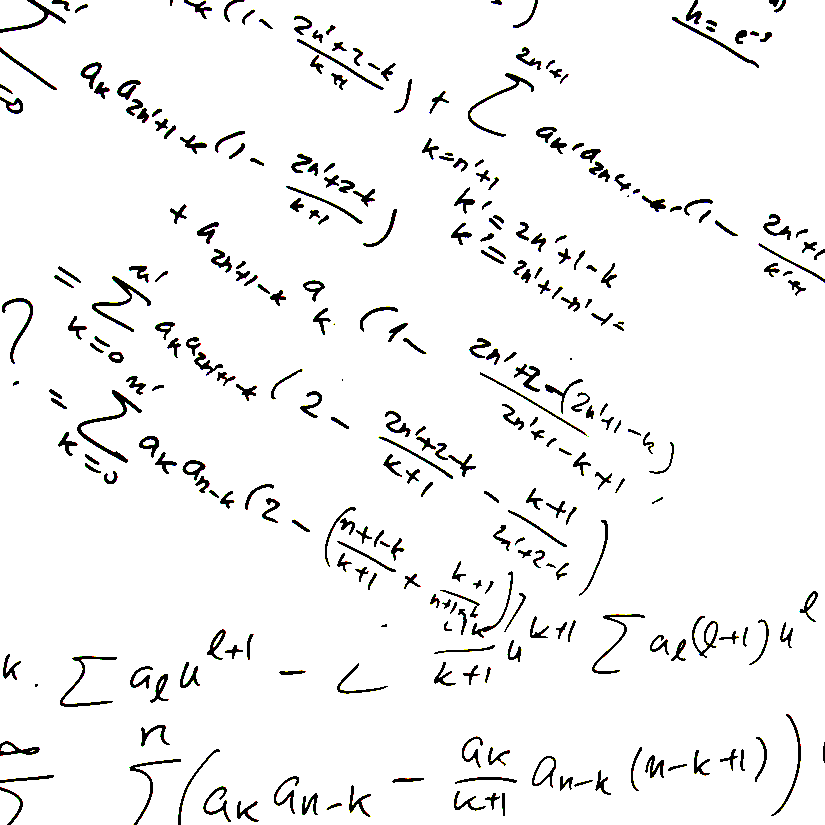
\includegraphics[width=8cm]{titlepic.png}
	};
\end{tikzpicture}
}

\usepackage[math]{iwona}

\newcommand{\hplus}{\mathbin{\hat+}}
\newcommand{\hdot}{\mathbin{\hat\cdot}}
% Описание теорем
\newtheorem{theorem}{Теорема}
\newtheorem{seq}{Следствие}
%%

%\VKR
\LECT % можно ещё лекцию забацать.
%\REPORT % можно ещё лекцию забацать.

%\titlepicture{
%%	\begin{tikzpicture}[overlay]
%%			\draw[opacity=0.4]  (-0.3,1.8) node {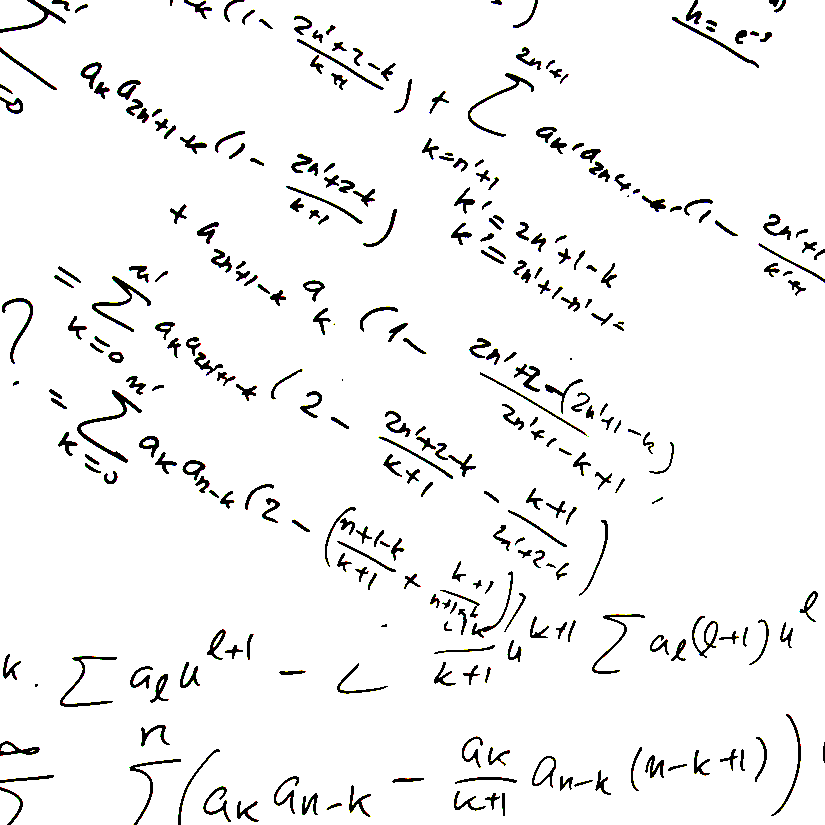
\includegraphics[width=3.5cm]{titlepic.png}};
%%	\end{tikzpicture}
%}

% Титульный лист теорем
\author[Д.\,В. Чупраков]{канд.\,физ.-матем.\,наук, доцент Д.\,В. Чупраков\\[6pt] usr10381@vyatsu.ru}

\institute[ВятГУ]{ФГБОУ ВО Вятский государственный университет}

\department{Факультет экономики и финансов}

\title[Лекция. Точечные и интервальные оценки]{
	Математическая статистика\\[12pt]
	Лекция. Точечные и интервальные оценкии--3}
\subtitle{Задача линейного программирования. Методы ее решения. Устойчивость}


\date{1 декабря 2020 г.}


%\setbeamercolor{coloredboxstuff}{fg=yellow,bg=white!10!blue}

\setbeamercovered{invisible}


\tikzset{
	 myarrow/.style={->, >=latex', shorten >=1pt, thick}
}



\tikzset{add/.style n args={4}{
    minimum width=6mm,
    path picture={
        \draw[black] 
            (path picture bounding box.south east) -- (path picture bounding box.north west)
            (path picture bounding box.south west) -- (path picture bounding box.north east);
        \node at ($(path picture bounding box.south)+(0,0.13)$)     {\tiny #1};
        \node at ($(path picture bounding box.west)+(0.13,0)$)      {\tiny #2};
        \node at ($(path picture bounding box.north)+(0,-0.13)$)        {\tiny #3};
        \node at ($(path picture bounding box.east)+(-0.13,0)$)     {\tiny #4};
        }
    }
}

\tikzset{bigadd/.style n args={4}{
    minimum width=20mm,
    path picture={
        \draw[black] 
            (path picture bounding box.south east) -- (path picture bounding box.north west)
            (path picture bounding box.south west) -- (path picture bounding box.north east);
        \node at ($(path picture bounding box.south)+(0,0.5)$)     { #1};
        \node at ($(path picture bounding box.west)+(0.5,0)$)      {#2};
        \node at ($(path picture bounding box.north)+(0,-0.5)$)        {#3};
        \node at ($(path picture bounding box.east)+(-0.5,0)$)     {#4};
        }
    }
}



\usepackage{mathtools}
\usepackage{pifont}
\newcommand{\verteq}{\rotatebox{90}{$\,=$}}
\newcommand{\equalto}[2]{\underset{\scriptstyle\overset{\mkern4mu\verteq}{#2}}{#1}}

\begin{document}


\maketitle

\begin{frame}{Структура лекции}
	\tableofcontents
\end{frame}


\section{Точечные оценки}

\begin{frame}[t]{}{}
\vspace{2cm}
{\LARGE Точечные оценки\par}
\vspace{\fill}

\end{frame}   

\subsection{Оценка параметра. Точечная оценка}

\begin{frame}{Оценка параметра. Точечная оценка}{}
\begin{tabular}{m{0.65\textwidth}m{0.33\textwidth}}
\structure{Определение}

 $\Phi$ \alert{Оценка параметра} - определенная числовая характеристика, полученная из выборки.
 

\end{tabular}

\structure{Определение}

Когда одно отдельное значение используется для оценки параметра, то такая оценка называется  $\Phi$ \alert{точечной оценкой генерального параметра} (средняя, дисперсия и пр.).

Всякая оценка является функцией результата наблюдений, т.к. чем больше и представительнее выборка, тем оценка будет более точной.

\end{frame}

\begin{frame}{Статистические оценки}{}
\begin{itemize}
	\item<1-> $\Phi$ \alert{Несмещенная} - математическое ожидание выборочного параметра при любых объемах выборки достаточно близко или совпадает с его генеральным значением.

	\item<2->  $\Phi$ \alert{Состоятельная} - с ростом числа наблюдений выбранная оценка стремится к истинному значению оцениваемого параметра (то есть дисперсия оценки стремится к нулю).

	\item<3->  $\Phi$ \alert{Эффективная} - дисперсия оценки имеет минимальное значение.
		
	\end{itemize}

\end{frame}   

\subsection{Генеральная и выборочная средняя}



\begin{frame}{Генеральная средняя}{}

\structure{Определение}
$\Phi$ \alert{Генеральной средней} (математическим ожиданием) дискретной статистической совокупности называется число, которое является центром рассеяния (варьирования) для всех значений изучаемого признака.

Генеральная средняя (теоретическая средняя) дискретного распределения находится как среднее арифметическое всех значений изучаемого признака:

$\mu = X=\frac 1 N \cdot\ \overset N{\underset{i=1}{\sum}}x_i $

или 
$\mu = \overset N{\underset{i=1}{\sum}}x_i \cdot \omega _i $ ,

где N - объем генеральной совокупности.
\end{frame}

\begin{frame}{Выборочная средняя}{}

\structure{Определение}
$\Phi$ \alert{Выборочная средняя} (математическим ожиданием) определяется как среднее арифметическое всех выборочных значений признака:


$$ 
    x=\frac 1 n \cdot\ \overset n{\underset{i=1}{\sum}}x_i 
$$
или, если значения отдельных вариант повторяются:

$$
     x=\frac 1 n \cdot\ \overset k{\underset{i=1}{\sum}}\left(n_i \cdot x_i \right),
$$

где $n$~--- объем выборки, k - количество отличающихся друг от друга вариант, $n_i$ -  количество значений $x_i$ вариант в выборке.

\end{frame}


\subsection{Генеральная и выборочная дисперсии}
\begin{frame}{Генеральная дисперсия}{}
\structure{Определение}
\alert{Генеральной дисперсией } называется величина, характеризующая степень рассеяния значений изучаемого признака относительно центра - генеральной средней или математического ожидания.

Генеральная дисперсия находится как среднее арифметическое квадратов отклонений всех значений изучаемого признака x_i в генеральной совокупности от генеральной средней X:

$ \sigma ^2_A=\frac 1 N \cdot\ \overset N{\underset{i=1}{\sum}}\left(x_i - \mu \right)^2 $, 
или, если значения повторяются: 

$ \sigma ^2_A=\frac 1 N \cdot\ \overset k{\underset{i=1}{\sum}}\left(x_i - \mu \right)^2 \cdot n_i $, 

N - объем генеральной совокупности, k - количество отличающихся друг от друга вариант, n_i - количество значений x_i в совокупности.
\end{frame}

\end{document}

\subsection{Генеральная и выборочная дисперсии}
\begin{frame}{Выборочная дисперсия}{}
\structure{Определение}
$\Phi$ \alert{Выборочная дисперсия } равна среднему арифметическому квадратов отклонений всех значений вариант выборки от выборочной средней:

Генеральная дисперсия находится как среднее арифметическое квадратов отклонений всех значений изучаемого признака x_i в генеральной совокупности от генеральной средней X:

$ \sigma ^2=\frac 1 n \cdot\ \overset n{\underset{i=1}{\sum}}\left(x_i - x \right)^2 $, 
\\или, если значения вариант повторяются: 

$ \sigma ^2=\frac 1 n \cdot\ \overset k{\underset{i=1}{\sum}}\left(x_i - x \right)^2 \cdot n_i $, 

\\n - объем выборки, k - количество отличающихся друг от друга вариант, n_i - количество значений вариант x_i в выборке.
\\Для оценки рассеивания выборки служит выборочное среднеквадратическое отклонение.
\end{frame}

  

\section{Интервальные оценки}
\begin{frame}[t]{}{}
\vspace{2cm}
{\LARGE	Интервальные оценка\par}
\vspace{\fill}

\subsection{Интервальная оценка}

\begin{frame}{Интервальнаяая оценка}{}
\begin{tabular}{m{0.65\textwidth}m{0.33\textwidth}}
\structure{Определение}

 $\Phi$ \alert{Интервальная оценка} - числовой интервал, определяемый двумя числами, содержащий неизвестный параметр генеральной совокупности. 
 
 \\Интервальная оценка более информативная, чем точечная оценка.  
 
 \\Если для произвольного числа \epsilon >0 выполняется неравенство |\Theta  - \Theta ^*|<\epsilon, то положительное число \epsilon характеризует точность оценки. В интервальной оценке устанавливается $\Phi$ \alert{доверительная вероятность \left(надежность \right), с которой эта оценка накроет неизвестный параметр, то есть это вероятность p, с которой выполяется неравенство |\Theta  - \Theta ^*|<\epsilon.
 
 \\Часто надежность принимают равной 0,9; 0,95; 0,99; 0,999.

\end{tabular}

\end{frame}

\subsection{Доверительный интервал}
\begin{frame}{Доверительный интервал}{}
\begin{tabular}{m{0.65\textwidth}m{0.33\textwidth}}
\structure{Определение}

 $\Phi$ \alert{Доверительным интервалом} называют найденный по данным выборки интервал \left (\Theta^*  - \epsilon; \Theta ^* + \epsilon \right) , длина которого равна 2\epsilon и является функцией результатов наблюдений.

\end{tabular}

\end{frame}


\subsection{Доверительный интервал}
\begin{frame}{Доверительный интервал для математического ожидания}{}
\begin{tabular}{m{0.65\textwidth}m{0.33\textwidth}}


 \\Доверительный интервал для математического ожидания при известном \sigma. В некоторых случаях квадратическое отклонение ошибки измерения, а вместе с нею т самого измерения бывает известно.
 
\\ Доверительный интервал для математического ожидания при неизвестном \sigma. Пусть случайная величина X имеет нормальное распределение с известными нам параметрами \mu и \sigma , и не зависящее от них. В этом случае используетсы распределение Стьюдента и интервальной оценкой математического ожидания генеральной совокупности с заданной надежностью p будет являться интервал 

$ \left(x - t_p\left(f\right)*\frac s \sqrt n ; x+t_p\left(f\right)*\frac s \sqrt n \right)$
\\с границей доверительного интервала \left(точность оценки \right) \epsilon = t_p\left(f\right)*\frac s \sqrt n .
\end{tabular}

\end{frame}


\subsection{Доверительный интервал}
\begin{frame}{Доверительный интервал для среднего квадратического отклонения}{}
\begin{tabular}{m{0.65\textwidth}m{0.33\textwidth}}


 \\Доверительный интервал для среднего квадратического отклонения \sigma. С надежностью p можно утверждать, что доверительный интервал \left(s - sq; s + sq \right) покрывает неизвестный параметр с точностью оценки \epsilon =sq . 

\end{tabular}

\end{frame}

\subsection{Примеры решения задач}
\begin{frame}{Примеры решения задач}{}
\begin{tabular}{m{0.65\textwidth}m{0.33\textwidth}}

$\Phi$ \alert{Пример 1:}
\\Случайная величина X имеет нормальное распределение с известным средним квадратическим отклонением \sigma =3. Найти доверительные интервалы для оценки неизвестноо математического ожидания \alpha по выборочным средним x, если объем выборки n = 36 и задана надежность оценки p= 0,95.
 
$\Phi$ \alert{Решение}
\\Найдем t. Из соотношения 2Ф\left (t \right) = 0,95 получим Ф\left( t \right) = 0,475. По таблице значений интегральной функции Лапласа находим t = 1,96. Найдем точность оценки \delta = \frac t*\sigma \sqrt n = \left(1,96*3 \right)/\sqrt 36 = 0,98. Доверительный интервал следующий: \left(x - 0,98; x + 0,98 \right). 

\end{tabular}
\end{frame}


\begin{frame}{Примеры решения задач}{}
\begin{tabular}{m{0.65\textwidth}m{0.33\textwidth}}

$\Phi$ \alert{Пример 2:}
\\При доверительной вероятности 90\%  найти доверительный интервал для D(x), если для выборки, объемом 5 выборочная D(x) = 6,6, а выборочная средняя 0,4.
 
$\Phi$ \alert{Решение}
\\По таблицам распределения \chi^2 найдем значение критерия \chi^2 для уровня значимости \upsilon =4 и \alpha =/2=0,05
\\ \chi^2_0,05;4=9,5
\\        \chi^2_\frac \alpha 2; \upsilon = \chi^2_0,95;4 = 0,711
\\ \frac 4*6,6 9,5 < \sigma^2 < \frac 4*6,6 0,711
2,78 < \sigma^2 < 37.13

\end{tabular}
\end{frame}


\begin{frame}{Примеры решения задач}{}
\begin{tabular}{m{0.65\textwidth}m{0.33\textwidth}}

$\Phi$ \alert{Пример 3:}
\\Признак X распределен в генеральной совокупности нормально. Найти доверительный интервал для \sigma с надежностью p=0,95 , если n=20, s=0,40.
 
$\Phi$ \alert{Решение}
\\Для надежности p=0,95 и n=20 найдем в таблице значений q=q\left( \gamma , n \right)  q=0,37. Далее s*q=0,40*0,37=0,148. Доверительный инетервал \left (0,40-0,15; 0,40+0,15 \right) , то есть \left( 0,25; 0,55 \right) покрывает \sigma с надежностью 0,95.

\end{tabular}
\end{frame}



\begin{frame}{Резюме}
	К настоящему моменту вы знаете:
	\begin{enumerate}
	\item 
		Точечную оценку 
	\item 
		Интервальную оценку
	\end{enumerate}
\end{frame}

\begin{frame}{Источники информации}
\begin{itemize}
\item 
	Статистические оценки параметров генеральной совокупности:  {\color{blue}\href{https://cloud.mail.ru/public/4SN3/2MJYgEz95}{Шилова З.\,В. , Шилов О.\,И.  Теория вероятностей и математическая статистика}} раздел 2 глава 2 с. 72--79, с. 88--90.
\end{itemize}

\end{frame}


\end{document}


